\section{Background}

\subsection{Electronic identity eID}

In Estonia, digital identity has been around for over 20 years \cite{eelaw-idcard}. The Estonian government issues ID cards loaded with certificates that enable cardholders to identify themselves digitally. Estonia's early adoption of eID, the political focus on digital government, has led to over 89\% of internet users accessing the e-government, making it the leading country in the EU \cite{eu-desi}. This adoption rate is in stark contrast to another EU country - Romania, where the first easy access to eIDs came in the form of new chip ID cards in August of 2021 \cite{romania-adopts-eid}. In that country, only 16\% of internet users access government services online. The adoption of eIDs in other countries lands somewhere between these two extremes.

It is clear that if a company wishes to implement eID authentication in a given country, it must realize the differences between the adoption rates. For some countries' citizens, the button "sign in with eID" will instinctively make them draw their smart card or other eID capable device, where it would confuse and repulse others. Depending on the country's market a company would like to access, eID sign-in may attract or repel potential clients. Early adopters must be aware of the widespread adoption of the eID infrastructure.

\paragraph{eID adoption in Estonia and Lithuania}

On the surface, Estonia and Lithuania have the exact eID solutions: Bank Link, ID card, Mobile-ID, and Smart-ID. However, even with the same infrastructure, we see many inconsistencies even in the case of just these two countries.

Consider Lithuania. It is possible to connect from a centralized website \url{https://epaslaugos.lt} to access the public sector services \cite{eidasnode-lt}. Here it is possible to sign in via bank link, ID card, and Mobile-ID. Smart-ID is not an option. The omission of Smart-ID is strange, as most banks support sign-in via three major eID providers, including Smart-ID, and actively encourage switching to it.

Some banks listed on the public sector gateway portal, like PaySera, provide significant security concerns. With that bank, it is possible to access the e-government services with only email, password, and a 2FA code sent to the registered person's phone number \todo{source: I did it myself 02-27}. For similar security concerns, Estonia's Information System Authority has taken steps to deprecate bank link \cite{ria-deprecates-bank-link} from use in TARA, Estonia's gateway to e-government.

In Estonia, all three major authentication options, ID card, Mobile-ID, and Smart-ID, can be used to access the e-government.

\subsection{eIDAS}

The eIDAS regulation \cite{eulaw-eidas} provided the groundwork for recognizing the signatures issued by other EU countries by imposing strict liability and mutual-recognition requirements. The regulation introduced the concept of a Trust Service Provider (TSP), which allowed relying parties to have a trust anchor. Before, with digital signatures, it was possible to verify that the person signed documents with a certificate and it was valid. However, there was no good way of ascertaining if a trusted authority issued the signing certificate. The role of establishing trust is the purpose of TSPs. Each member state maintains a list of their TSPs, where each TSP is certified to perform specific tasks, such as timestamping or issuing signing certificates.

The regulation also requires member states to establish eID systems and integrate them into a federal plan if they haven't already. This regulation was also the basis for creating the eIDAS node network \cite{carretero2018federated}. These nodes connect across country borders, allowing users to authenticate with the eID of their home (eID issuer) country in the host (current residence) country. The eIDAS authentication protocol redirects the authentication requests to the appropriate country, federating the identification process. For the institutions trying to target the EU market, this provides a significant advantage since access to one node would mean access to all nodes in the EU.

The main issue private companies encounter when accessing the network is the highly exclusive access. The eIDAS network is only concerned about connecting countries. How and who can access an eIDAS node is up to the member states to decide.

\paragraph{eIDAS notifications in Estonia and Lithuania}

For countries to communicate through the eIDAS node network, the governments must first notify the European Commission about what eID authentication methods they will provide \cite{eulaw-eidas}. Other countries can then use these methods to authenticate foreign citizens into their public services.

In the case of Estonia, the country has notified the European Commission about its smart card and Mobile-ID authentication methods \cite{eulaw-eidas-notified}. Smart-ID is not a permitted method of authentication in the context of eIDAS. In Lithuania's case, only the smart card solution is allowed - no mobile sign-in methods have been notified \cite{eulaw-eidas-notified}.

The governments of these two countries have revealed a gap of what they consider to be a secure and trusted source of eID and what they are willing to be held liable for in the context of the eIDAS network.

\subsection{eID providers in Estonia}

Applied Cyber Security Group of the University of Tartu maintains a list of e-services \cite{ut-eidinestonia} that uses at least one eID authentication method in Estonia. The following authentication methods were listed: Bank Link, ID-card, Mobile-ID, Smart-ID, TARA, and HarID.

While the list does not count Dokobit and eeID as primary eID providers, they list them as consumers of at least of schemes mentioned before. Their business model is to act as an intermediary for ease of integration.

\subsubsection{Bank link}

Banks have initially created this authentication method to provide close integration with e-commerce providers to receive risk-free payments \cite{kerem2003internet}. Over time it saw an additional use case - secure and trustworthy authentication method for the public and private services \cite{sebbanklink}.

Researchers found that the bank link protocol, while applicable, was "extremely insecure" \cite{banklinksecurityanalysis}. From March of 2021, RIA has disabled the use of bank link to access public services \cite{ria-deprecates-bank-link}, which accounted for only 1 percent of all authentications, also revealing its popularity in public.

Due to the lack of security auditing required to satisfy eIDAS, poor market reach, and no support from the government, this authentication method will not be discussed in the scope of this thesis.

\subsubsection{Smart card (ID card)}

ID cards are the most popular way to access their eID in Estonia, primarily due to the legal requirement of having one. The Identity Documents Act \cite{eelaw-idcard} states that all EU, not only Estonian, citizens residing in Estonia must hold an ID card, with which they could access public services online. Interestingly, this requirement caused the government to issue more ID cards than there are people in Estonia \cite{ria-idee,statee-population}. Smart card functionality touches not only ID cards but residence permits and other government-issued cards as well \cite{eulaw-eidas-notified}.

There are no variable costs to allow a person to log in to websites with their smart card. For this authentication method, no per-transaction fees exist, as the certificate validity service (OCSP) \cite{rfc6960} can be queried for free.

An end user's computer can extract an authentication certificate from their smart card with the help of special software, generally distributed by the government agency responsible for maintaining the cards \cite{ria-idee}. This certificate, once on the computer, can be sent to the private company's authorization server with Client Certificate TLS option \cite{rfc8446} natively or with the use of specialized helper library \cite{ria-webeid}, using standard REST calls.

Qualified trust service provider for Qualified Certificates for e-signatures installs the certificates in ID-cards \cite{eu-trustservices}, which ensures a high degree of certainty about the identity of the person authenticating.

A significant advantage of using a decentralized eID infrastructure, such as ID card authentication, is that there is no intermediary service in the process, allowing companies to skip going into expensive contracts with an eID service provider.

\subsubsection{Mobile-ID}

Five years after SK ID Solutions introduced ID cards for use in Estonia, they have developed a mobile phone-friendly way to access the users' eID for use in Estonia and Lithuania \cite{sk-history2007}. SK achieved it by extending the functionality of phone SIM cards by adding new applications on the microchip.

The price of using Mobile-ID for the service provider varies based on usage, starting from 10 euro per month (10ct per request) to costing over 5 000 euro, where the effective cost is under 1ct for request \cite{sk-mobileidpricing}. For the end-user, mobile operators can charge an additional fee for the use of this service \cite{telia-mobileid}.

Accepting Mobile-ID would allow companies to access the markets of two countries: Estonia, and Lithuania, as the technical implementation is identical.

Qualified trust service provider for Qualified Certificates for e-signatures installs the certificates in a particular variety of SIM cards, capable of supporting Mobile-ID \cite{eu-trustservices}, which ensures a high degree of certainty about the identity of person authenticating.


\subsubsection{Smart-ID}

Smart-ID is the latest and fastest-growing way of accessing citizens' eID, working in all 3 of the Baltic States \cite{sk-history2017}. The protocol utilizes mobile phones as authentication, similar to Mobile-ID. Unlike Mobile-ID, it does not require specialized external hardware \cite{smartid-docs}. The authentication process is handled by combining the eID server and the end user's smartphone. Despite that, it still passed the eIDAS compliance audit for the requirement of ensuring signature private key is "with a high level of confidence under sole control" of its owner \cite{enisa-eidasreq}. After passing the audit, Smart-ID was recognized as a QSCD, allowing it to create QES in 2018 \cite{smartid-qscd}.

The price of using Smart-ID for service providers, much like Mobile-ID, varies based on usage, starting from 50 euros per month (10ct per request) to over 20 000 euros, where the effective cost is under 1ct for request, based on the total amount of transactions performed within a month \cite{sk-smartidpricing}. For users, unlike Mobile-ID \cite{telia-mobileid}, there are no telecommunication operators involved, and there are no additional costs.

Implementation of Smart-ID would allow users to access the markets of three countries: Estonia, Latvia, and Lithuania.

Qualified trust service provider for Qualified Certificates for e-signatures users their data centers to hold part of the private key and certificate used to authenticate users \cite{eu-trustservices}, which ensures a high degree of certainty about the identity of person authenticating.

\subsubsection{TARA}

TARA is Estonia's primary gateway for authentication to public services \cite{tara}. TARA provides the ability for users to sign in with any of the three primary eID methods of Estonia and with the eID schemes of other EU member states. The ability to authenticate with the systems of other countries is of particular interest, as it also doubles up as the official eIDAS node of Estonia \cite{tara}.

Estonian Information System Authority intends to limit the use of TARA to public services only \cite{tara-business}.

Technical implementation for the consumer, unlike Mobile-ID and Smart-ID, will be much easier to implement, as it uses the well-adopted protocol of OpenID Connect \cite{tara-technical, oidc}.

It is worth mentioning while the underlying authentication methods have received proper eIDAS auditing and are backed by a qualified trust service, this and all of the following authentication methods have not been audited in compliance with eIDAS, or the auditing was not made public.

TARA only acts as an authentication service. It would not be able to provide means of signing documents \cite{tara-technical}. If the business is considering expanding to allow for online digital signing, an infrastructure like TARA will unlikely be a great choice.

\subsubsection{eeID}

Estonian Internet Foundation created eeID service for the exclusive purpose of bringing eID authentication to the private sector \cite{eeid}. It is a clone of TARA without it being Estonia's gateway for the eIDAS node network. The similarities mean that all points outlined to TARA apply to this service too.

The service is new, does not have pricing tiers, and currently asks for 9ct per successful authentication request \cite{eeid-pricing}.

The vision of the said service is to allow users to access the markets of all EU countries. Currently, there are only fourteen countries with notified eID authentication methods \cite{eulaw-eidas-notified}: Estonia, Germany, Italy, Spain, Belgium, Luxembourg, Croatia, Portugal, Latvia, Lithuania, Netherlands, Czech Republic, Slovakia, and Denmark.

\subsubsection{HarID}

Estonian Ministry of Education and Research created this service for the youth of Estonia to access different educational institutions across Estonia \cite{harid}. ID cards are only legally required to be held by citizens over the age of 15 \cite{eelaw-idcard}, so everyone under would have been unable to access their school system. HarID accepts TARA authentication methods with the addition of username \& password. This authentication method is held exclusively for the education sector and will be skipped over in this thesis.

\subsubsection{Dokobit}

In the initial list of services using eID in Estonia \cite{ut-eidinestonia}, one service stands out - Dokobit \cite{dokobit}. They provide services comparable to eeID in that they aggregate different eID methods of Estonia (ID-card, Mobile-ID, and Smart-ID) and other countries. The primary difference between the two authentication providers is how they want to achieve their multi-national implementation goal. Dokobit relies on integrating each country's system individually. In contrast, eeID depends on using the framework of the eIDAS infrastructure \cite{eeid}.

Pricing for Dokobit varies drastically, and the provided prices for the Baltic States \cite{dokobit-pricing} start at 50 euros per month (7.1ct per request), going down to 4.2ct per request at 500 euros per month.

Dokobit supports 11 countries: Estonia, Italy, Spain, Belgium, Latvia, Lithuania, Finland, Norway, Iceland, Poland, and Portugal \cite{dokobit}.

UAB Dokobit is a trust service provider for Qualified validation of qualified e-signature. It means the service itself does not provide Digital Signature certificates, but eIDAS considers the results of validation of signatures trustworthy \cite{eu-trustservices}.

\subsection{Authentication and QSCD}

The requirements for Estonian ID cards make a clear distinction between "ADF AWP" and "ADF QSCD" applications. Both software applications are loaded onto the smart card; however, only the QSCD application, guarded by PIN2, can create QES. Implication here is that for authentication with an ID card, a QSCD is not used.

The fact that smart cards do not use a QSCD for authentication does not mean that the certificate used was not audited under eIDAS. In practice, the same QTSP CA issues both the authentication and the QSCD certificates (see figure \ref{fig:est-id-sameissuer}). "Since the authentication certificate is issued under the same CA and the same Terms and Conditions, the certificate policy documents and other CA statements are applicable to both certificates" \cite{arnis-phd}. While eIDAS does not outline any requirements for authentication modules in the QSCDs, it is reasonable to assume that the QTSP took the exact organizational and technical measures to protect the authentication key on the same physical device.

\begin{figure}
    \centering
    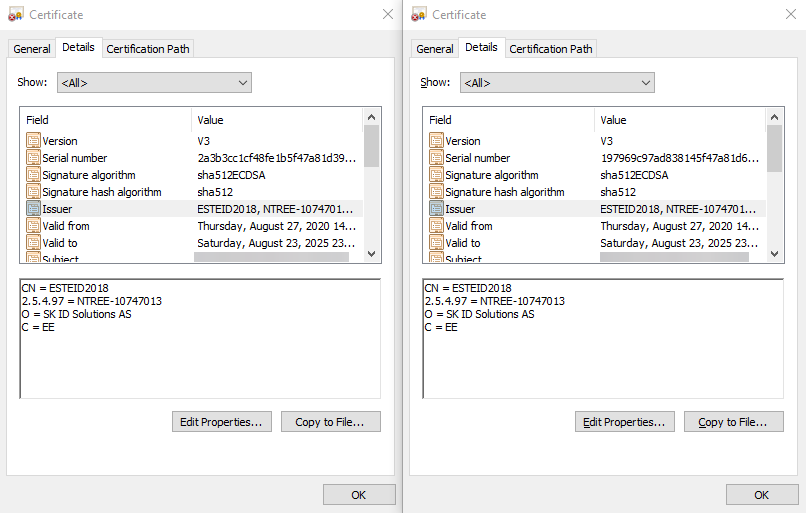
\includegraphics[scale=0.69]{est_id_sameissuer}
    \caption{Comparison of authentication (left) and signing (right) certificate issuer field}
    \label{fig:est-id-sameissuer}
\end{figure}

For different eID authentication schemes, companies have to assess the scheme's security on a case-by-case basis. For all of the methods analyzed in the thesis (Lithuanian and Estonian ID cards, Mobile-ID, and Smart-ID), the same QTSP signed both certificates - for authentication and signing. There seems to be no discernable benefit to issuing an authentication certificate with a different CA, so if a device offers both authentication and qualified signature creation functionality, it is highly likely that the authentication certificate is as trustworthy as the eIDAS compliant QSCD.

\paragraph{Special case: third-party providers}

When using an intermediary such as TARA (eeID) or Dokobit, the new eID provider acts as a new trust anchor. All rigorous eIDAS and QTSP auditing become irrelevant when using intermediary services, as systems are as secure as their weakest links. Companies must first look at the security auditing and the certifications of the intermediary; only then consider the security of authentication options its delegates.

\subsection{Levels of assurance}

The eIDAS regulation uses three assurance levels: low, substantial, and high. These levels refer to the degree of confidence about the claimed or asserted identity of a person \cite{eulaw-eidas}. These assurance levels map to levels 2-4 of ISO 29115 \cite{iso29115}.

\TODO{Finish this section}

% It is important to make that the security requirements for a certain level of assurance are only a prerequisite. 
% https://eur-lex.europa.eu/legal-content/EN/TXT/PDF/?uri=CELEX:32015R1502&from=EN

\subsection{GDPR}

When dealing with eID, sensitive personal data processing is required. Two years after the EU enacted the eIDAS legislation, the parliament issued new legislation to consolidate all previous privacy laws \cite{eulaw-gdpr}.

In GDPR, companies must be aware of key terminology. Interested parties can find a complete list of definitions in article 4 of the regulation. Below you can see a list of the most critical keywords in the context of eID authentication.

\paragraph{Personal data} The eID solutions in scope all provide the following personal information: full name, serial number (national id), and the country of origin.

\paragraph{Processing} The minimal amount required to process information is to store uniquely identifying information that would link an eID to an internal id code. At the very least, this action involves collecting, storing, and retrieving personal data.

\paragraph{Processor and Controller} In the minimal case, no third parties are involved, and the controller, the processor, and recipient are the same entity.

\subsection{Threats}

\TODO{There has to be a source with the extensive list, all protocols I checked look the same, but I can't seem to find a post saying yes, you need to do this.}

\begin{figure}
    \centering
    \begin{sequencediagram}
        \newthread{A}{Natural Person}{}
        \newinst[1]{B}{Relying Party}{}
        \newinst[1]{C}{QSCD Interface}{}
        \newinst[2]{D}{QSCD}{}

        \begin{call}{A}{authenticate()}{B}{Auth token}
            \begin{call}{B}{authenticate()}{C}{Certificate + authenticity proof}
                \begin{sdblock}{Block}{Outside of RP control}
                    \begin{call}{C}{getCertificate()}{D}{Client Authentication certificate}\end{call}
                    \begin{call}{C}{signChallenge()}{D}{Signed challenge}
                        \begin{call}{D}{enterPin()}{A}{PIN}\end{call}
                    \end{call}
                \end{sdblock}
            \end{call}
            \begin{call}{B}{validateResponse()}{B}{}\end{call}
        \end{call}

    \end{sequencediagram}
    \caption{High-level sequence diagram of a eID authentication flow}
    \label{fig:eid-auth-flow-seq}
\end{figure}

In the sequence diagram (see figure \ref{fig:eid-auth-flow-seq}), we see a high-level overview of any eID authentication solution. In the authentication protocol, the relying party (company implementing eID sign-in) entirely depends on the QSCD interface, which acts as a trust anchor. A communication channel exists between the relying party and the interface. We can categorize the channel type into two groups:

\begin{enumerate}
    \item trusted, where the sender can reasonably guarantee that adversaries are unable to change the data in transit (Smart-ID, TARA, Dokobit);
    \item untrusted, where there is a reasonable possibility for data to be tampered with in transit (Web eID).
\end{enumerate}

Trusted communications generally operate using an encrypted backchannel, where untrusted ones require the client to send data from the QSCD interface. Because the client sends the data, this becomes an untrusted channel, and the relying party must perform additional certificate verification.

Failure to encrypt and establish the authenticity of the interface in a trusted backchannel or not validating data in an untrusted channel allows adversaries to perform man-in-the-middle attacks.

\TODO{Limitations: For the scope of the thesis, only two security aspects will be analyzed: the network communication between the natural person and the interface and the certificate authenticity guarantees. Security analysis of QSCD and its communications with the interface will not be analyzed.}

\TODO{Further research? Limitations: proper analysis of what companies would like to see in a solution for more accessible bullet points}